\section{Localised Processing, Storage and Classification}
In this section the report will discuss the implementation of the edge node and all facilities within it.
\subsection{Setting up the Environment}
In order to simulate an edge Device rather than a separate piece of hardware, a Virtual Machine (VM) can be setup on the laptop. However, the virtual machine is just to represent an edge device running an embedded UNIX OS. In this scenario using Vagrant in conjunction with VirtualBox allows for the setup and use of a virtual Ubuntu system. This is all to emulate an edge device such as a Raspberry Pi or a server running at the remote location. The guide on the Vagrant website takes the developer step by step through the stages of getting the VM setup. \cite{installing_vagrant}. 

Once this is setup, the Greengrass Core (GGC) can now be initiated and ran on the \textit{Edge Device}. First the Greengrass group was created via the IoT Core page on AWS and then a group was setup using the default settings. When the group is first initialised, a zip file filled with correct certifications and configuration files is produced. These files must be placed into the installed GGC folder on the Edge Device under \textit{/greengrass/certs} and \textit{/greengrass/config}. Then the Greengrass Core can be started up by running the program stored at \textit{/greengrass/ggc/core/greengrassd}. Upon doing this, the message shown in Figure \ref{fig:running_greengrass_on_vm} will appear showing that the Greengrass Core has successfully launched and deployments will then begin running. 

\begin{figure}[ht]
    \centering
    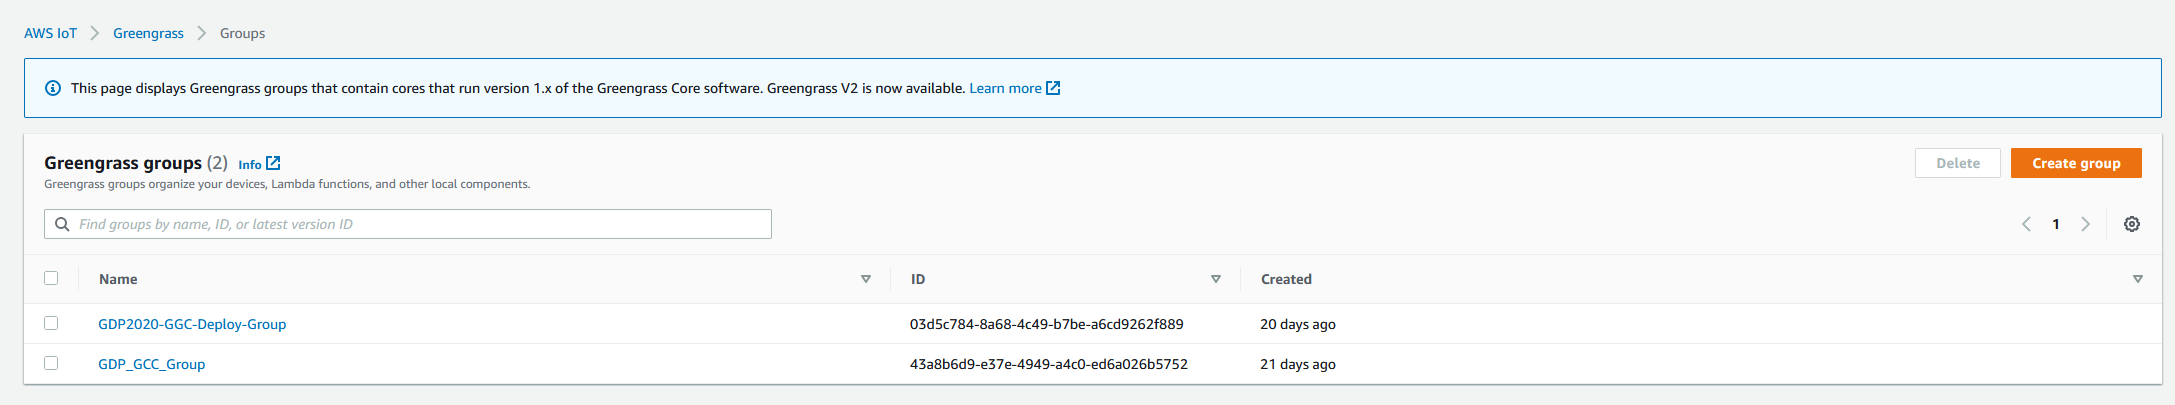
\includegraphics[width=1\linewidth]{pages/Chapter4/Chapter 4 Images/greengrass_group.png}
    \caption{Setting up Greengrass Group on the AWS IoT Core dashboard}
    \label{fig:my_label}
\end{figure}
\begin{figure}[ht]
    \centering
    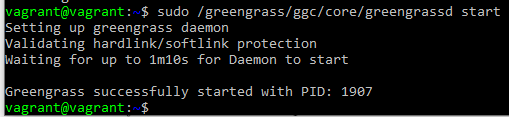
\includegraphics{pages/Chapter4/Chapter 4 Images/correctly_starting_greengrass.png}
    \caption{Deploying and Running Greengrass on the VM}
    \label{fig:running_greengrass_on_vm}
\end{figure}

There are then some additional steps that need to be run for installing the pre-requisites and give the Greengrass Group, access to run its runtime and the Greengrass daemon. The pre-requisites are specifically the Lambda run-times required (e.g. for Python or NodeJS). These instructions and the specific commands can be found in the AWS Documentation in Greengrass Deployment \cite{greengrass_deployment}.

\subsection{Attaching Lambda Functions to the Greengrass Group}
Once the Greengrass Group is established, a Lambda function to run on the device can be setup as long as the runtime requirements are also on the device (e.g. nodejs12.x must be installed to run NodeJS at the edge device). Then on the Greengrass Group dashboard a new existing Lambda function is attached, as shown in Figure \ref{fig:adding_new_lambda_to_ggc}. The first step is to add the Lambda function, then attach an existing Lambda function from the provided list. This Lambda function must already have been created in the AWS Lambda Dashboard.

\begin{figure}[ht]
    \centering
    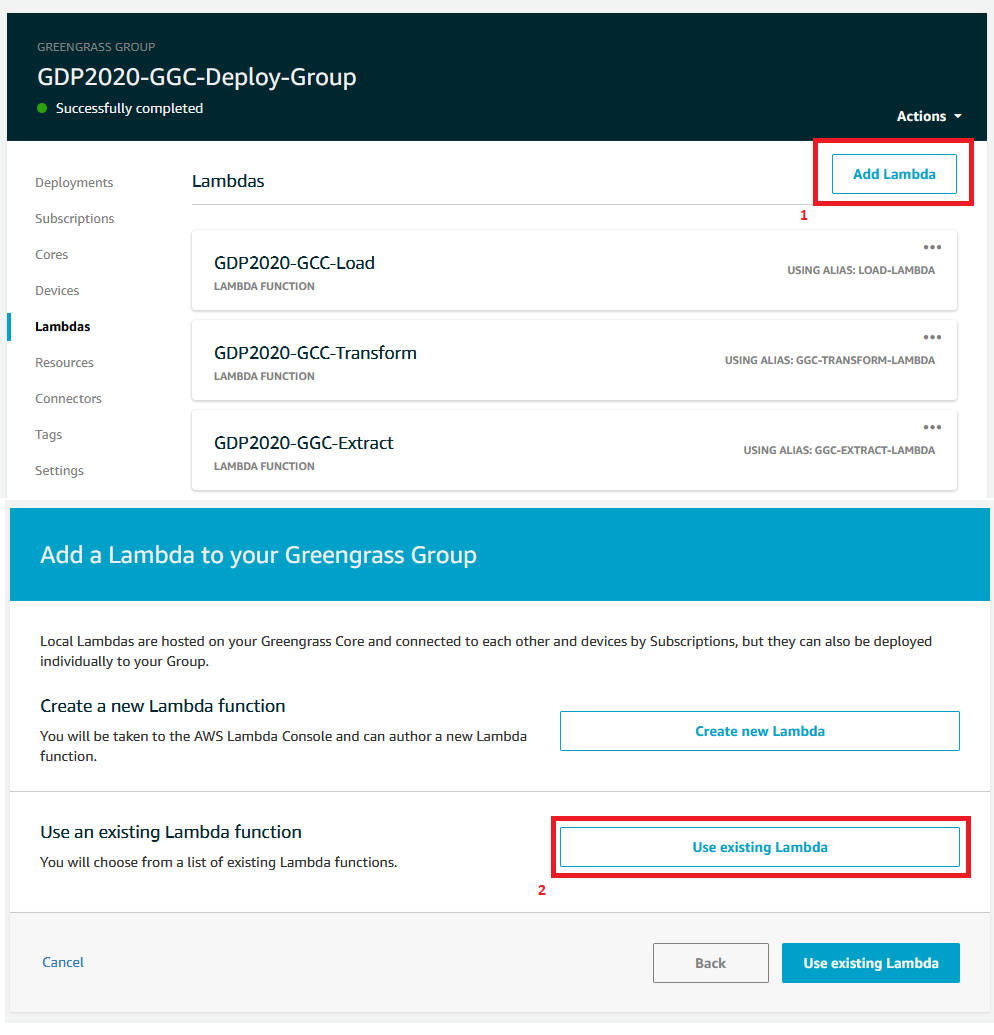
\includegraphics[width=0.7\linewidth]{pages/Chapter4/Chapter 4 Images/greengrass_new_lambda.png}
    \caption{Adding a new Lambda Function via the Dashboard.}
    \label{fig:adding_new_lambda_to_ggc}
\end{figure}

Once this is complete, the drop down in the top right of the Greengrass Groups dashboard allows you to deploy or re-deploy an existing version, as shown in Figure \ref{fig:deploy_on_dashboard}.

\begin{figure}[ht]
    \centering
    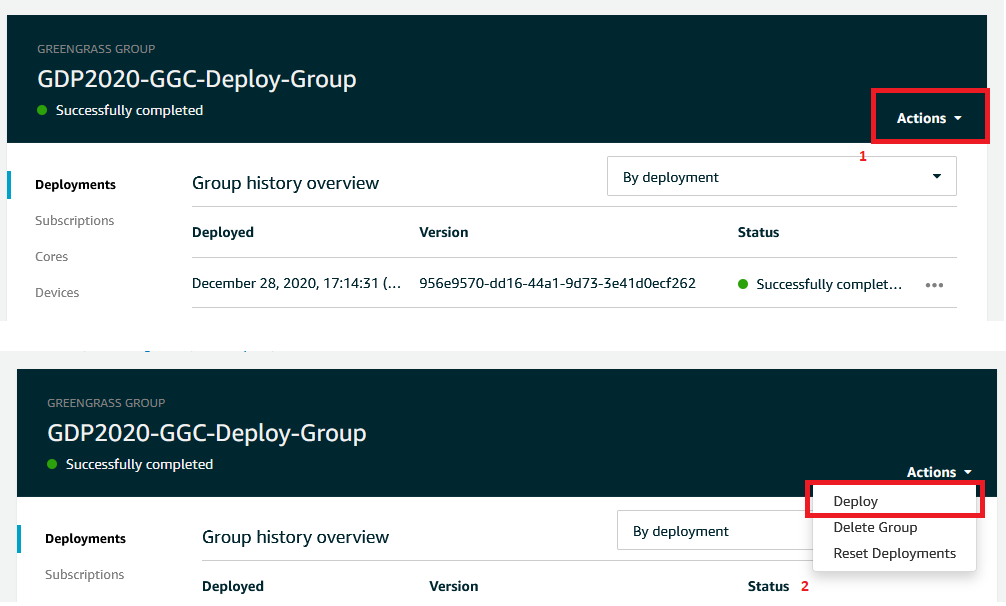
\includegraphics[width=0.7\linewidth]{pages/Chapter4/Chapter 4 Images/deploy_group.png}
    \caption{How to deploy the Greengrass Group via the Dashboard}
    \label{fig:deploy_on_dashboard}
\end{figure}


To enable the GGC to access the hosts' local resources, \textit{Local Resource Access} must be setup on the group. Local Resource Access is a way for the containerised Greengrass Core to gain access securely to a specific directory outside of the container. This is done by setting up a \textit{src} directory on the host, and a matching \textit{dest} directory on the Greengrass device. This process can be seen in Appendix \ref{appendix:ggc_lra}. A folder within the containerised GGC is labelled as \textit{'dest/LRAtest/...'} and outside of the container on the host device (or VM for this project) is a similar folder \textit{'src/LRAtest/...'}. These two directories are linked with each other. Files stored into the former location will be also seen on the host machine under the latter location and visa versa.

The next following sections will discuss how to setup each Lambda function.
\begin{itemize}
    \item Extract - \ref{extract_fn_impl}
    \item Transform - \ref{transform_fn_impl}
    \item Load - \ref{load_fn_impl}
    \item Local ML Inference - \ref{load-ml-fn}
    \item Remote ML Inference - \ref{remote-ml-fn}
    \item NodeJS Web Server Application - \ref{nodejs-server}
\end{itemize}


\subsection{Extract Function}
\label{extract_fn_impl}
The first localised Lambda function, the Extract function, collects any .db files from the End-user's device and begins processing it at the Edge. This frees up the End-user's device for other tasks as previously explained. As this is the first documentation of Lambda Function implementation, one requirement to run any function is to include the Greengrass SDK. This is done by uploading a zip file to the Lambda function which includes the main program file and the SDK Folder as seen in Figure \ref{fig:ggc_sdk_inclusion}
\begin{figure}[ht]
    \centering
    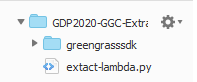
\includegraphics{pages/Chapter4/Chapter 4 Images/LambdaFns/ggc_sdk_inclusion.png}
    \caption{How the zipped  directory needs to be uploaded.}
    \label{fig:ggc_sdk_inclusion}
\end{figure}

This setup must be completed for each function, and any external Python dependencies must also be included in this zip file. Once the setup is complete, then the Python application can be developed. The extract-function Python implementation follows the data-flow shown in Figure \ref{fig:lambda_extract_fn}.

\begin{figure}[ht]
    \centering
    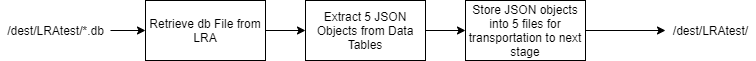
\includegraphics[width=1\linewidth]{pages/Chapter4/Chapter 4 Images/LambdaFns/extract-fn.png}
    \caption{Extract Lambda Function Block Diagram}
    \label{fig:lambda_extract_fn}
\end{figure}

The implementation for this function is very similar to the implementation for the Laptop-To-Cloud pipeline with the main changes being the setup required for the local resource access from the edge node.

\subsection{Transform Function}
\label{transform_fn_impl}
The transform function implementation follows the block diagram shown in Figure \ref{fig:lambda_transform_fn}, with the main points being where the output file and the compressed JSON object with all the separate data tables' data in one is placed. The output file is placed into three locations for usage by other Lambdas. It should be noted that it was chosen to replicate the three output files so as to avoid any issues with access from multiple locations (separate Lambda functions). However, this leads to a longer run-time as the write operation has to be run three times rather than once, but is only a problem for very large files as is seen later in the testing stages.

\begin{figure}[ht]
    \centering
    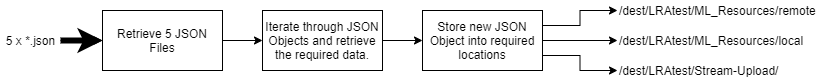
\includegraphics[width=1\linewidth]{pages/Chapter4/Chapter 4 Images/LambdaFns/transform-fn.png}
    \caption{Block Diagram of Transform Function at the Edge Node}
    \label{fig:lambda_transform_fn}
\end{figure}


\subsection{Load Function}
\label{load_fn_impl}
For this Lambda function, the Python library \textit{requests} is used and so the dependency folder must be extracted from several ways. 
\begin{itemize}
    \item Copy directly from developer's Python dependencies list.
    \item Setup a virtual environment for Python and install all dependencies, this will then be stored locally in that virtual environment. These can then be zipped up and extracted and the developer's program injected into the zipped folder for upload to the Lambda function.
\end{itemize}

The requests library is small with no build requirement (this will become an issue later for the XGBoost library). The required directory was copied directly from the developer's Python-libraries list after using \textit{pip install requests} and \textit{pip show requests} to ensure no other sub-dependencies were required. The latter command also showing where this installed requests library can be found so as to be copied. The final zipped folder to upload to the Load-Lambda function is shown in Figure \ref{fig:lambda_requests_ggc_sdk}.

\begin{figure}[ht]
    \centering
    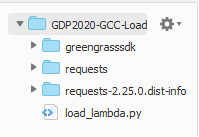
\includegraphics{pages/Chapter4/Chapter 4 Images/LambdaFns/ggc_sdk_requests_inclusion.png}
    \caption{File structure for Upload to Load Lambda with Requests and GGC SDK}
    \label{fig:lambda_requests_ggc_sdk}
\end{figure}

The implementation of the load Lambda function follows the block diagram in Figure \ref{fig:lambda_load_fn}. Environment variables can also be setup within the AWS Lambda dashboard to ensure no details of the private key are released without intention. 

\begin{figure}[ht]
    \centering
    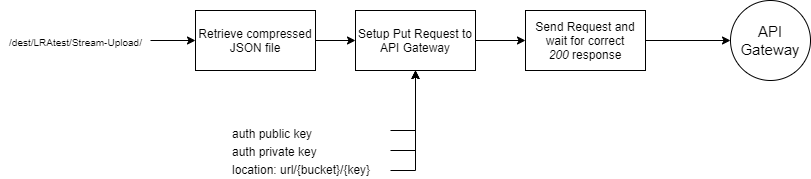
\includegraphics[width=1\linewidth]{pages/Chapter4/Chapter 4 Images/LambdaFns/load-fn.png}
    \caption{Block Diagram of Load Function at the Edge Node}
    \label{fig:lambda_load_fn}
\end{figure}


\subsection{Local-ML Function}
\label{load-ml-fn}
%looooooooooooong%
For the Local-ML Lambda function setup there are several steps that need to be completed. \begin{enumerate}
    \item Import the Sagemaker Model from either Sagemaker or S3.
    \item Setup Python Dependencies for use of XGBoost Python Library at the edge, these must be built specifically for the end-device architecture and OS. (e.g. Linux on x84\_64 architecture).
    \item Upload zipped file of Dependencies and Python program file.
    \item Complete program and deploy to Greengrass Core.
\end{enumerate}
These four stages describe the implementation process, with the second stage being the most difficult and time consuming. This is because the XGBoost Python package and its sub-dependencies must be built from source due to usage of C program files within XGBoost, and these must be built for the target device. 



The first stage of this setup procedure is as follows. In the development stages of Sagemaker Model Training and Deployment, a model is produced as a zip file. This zip file containing the ML-Model can be imported direclty into the Greengrass Group as a resource to be used within the container environment. It can be either imported from S3 or directly from Sagemaker. This is seen in Figure \ref{fig:ggc_model_import} where the ML model must also be attached to a Lambda function for it to be accessible by that Edge-based Lambda function. First the \textit{'Add machine learning resource'} must be clicked, then the model name entered and a choice must then be made for the source location of the model. As shown in Figure \ref{fig:ggc_model_import}, the model is uploaded from a provided S3 bucket and location within it. Then the local path within the Greengrass container is also chosen. This is for usage within the attached Lamda function to the Machine Learning Resource, to open the directory with the model.

\begin{figure}[ht]
    \centering
    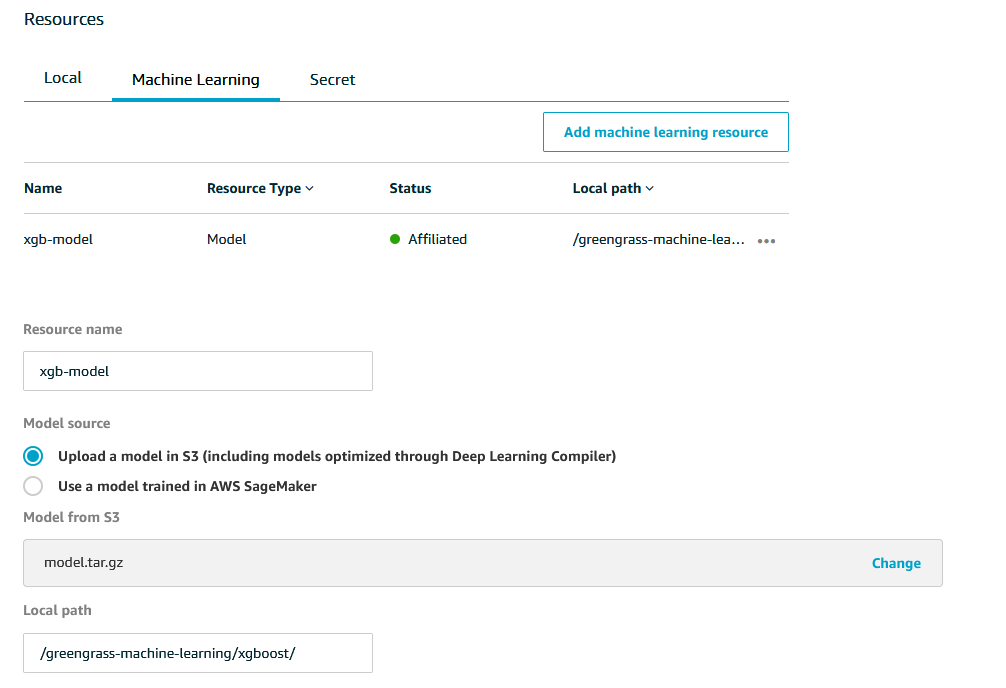
\includegraphics[width=1\linewidth]{pages/Chapter4/Chapter 4 Images/LambdaFns/xgboost_model_import_ggc.png}
    \caption{Importing XGBoost Model from S3 into the Greengrass Group as a local Resource}
    \label{fig:ggc_model_import}
\end{figure}

Once the ML-Model is attached and a Lambda function to handle the Local-ML Inference is also attached, then the dependencies can be built. First an EC2 instance is instantiated in order to help the developer build and pack the dependencies. The developer must set up a \textit{virtual Python environment} so that the Python dependencies are installed remotely and any sub-dependencies are also present (as these must also be zipped as previously mentioned). The developer must then also install Python 3.7 rather than Python 3.8 within the Virtual environment as Greengrass at the time of writing this report only supports Lambda functions with a runtime of Python 3.7. Once the \textit{virtual Python environment} is setup and any sub-depencies or other required libraries are also installed within. In this case, the dependencies required are:
\begin{itemize}
    % \item \textit{xgboost}
    \item \textit{numpy}
    \item \textit{scipy}
    \item \textit{six}
    \item \textit{pkg\_resources}
\end{itemize}
Once these dependencies are setup, download the XGBoost source files from GitHub and use CMake to manually compile the program for the Amazon Linux OS running on x86\_64 architecture. It should be noted that CMake will also need to be downloaded and compiled from scratch. The exact commands to achieve this can be found on a post by Lucas Silva \cite{silva_2019}. However, these commands must be adjusted for this project's specific sub-dependencies, and the article uses Python 3.8 rather than 3.7, to install Python 3.7 it requires further adjustment of the commands as seen in the article by Rahul Kumar for installing Python 3.7 on Amazon Linux. \cite{kumar_2020} 

Following the instructions provided produces a zip file that can be uploaded to an S3 bucket for retrieval from the EC2 instance and then uploaded into Lambda. Once this is complete the implementation of the program can begin. The implementation of the main program follows the block diagram shown in Figure \ref{fig:localml-function}. The block diagram shows how the program running in the Lambda function will operate. First it must retrieve the model and the JSON file from the appropriate local directories in the Greengrass container. Then apply some pre-processing to make them fit for usage. The XGBoost Python package then comes with a predict function that allows us to input the data parameters for one timestamp and per MAC Address. This output result can then be stored locally, passed to the OTT Application or to the Web server application for live-viewing of the results, as well as for comparisons to the Remote-ML timings.

\begin{figure}[ht]
    \centering
    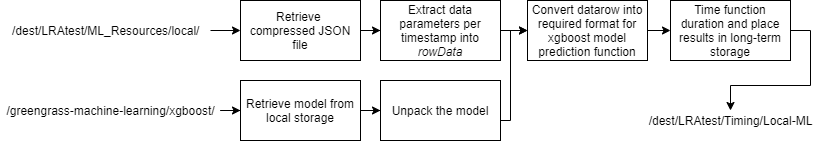
\includegraphics[width=1\linewidth]{pages/Chapter4/Chapter 4 Images/LambdaFns/localml-fn.png}
    \caption{Block Diagram for Local-ML Function at the Edge Node}
    \label{fig:localml-function}
\end{figure}
%Import of Sagemaker model into greengrass via dashboard
%How it can be accessed
%Setup of Dependencies using Cloud-Based resources, ensure version for python3.7, ensuring also size of lambda zip is less than 250mb as a hard limit from them
% any more than 50mb must be uploaded from s3

\subsection{Remote-ML Function}
\label{remote-ml-fn}
Once the requests library is correctly packed with the Lambda program file. As well as the API Gateway setup to trigger a Lambda function, which in turn will trigger the Sagemaker Endpoint. A similar implementation as seen in Figure \ref{fig:lambda_load_fn} is used, however the URL used in the HTTP request will be different. The response from the endpoint is also how the Lambda function will receive the results of the Machine Learning Model's output. A code snippet shows how the request can be setup by reading the JSON file and then sending the data as requested to the API Gateway to be processed by the Cloud-Based Lambda as shown in Listing \ref{lst:edge_remote_ml}
\begin{lstlisting}[language=Python, caption={Sending Data to API Gateway to Invoke Cloud-Based Lambda for Sagemaker Endpoint}, label={lst:edge_remote_ml}]
with open(jsonLoc, 'r') as jF:
                payload = json.dumps(json.loads(jF.read()), separators=(',',':'))
            client.publish(
                topic='mlEndpoint/checkFile', 
                queueFullPolicy='AllOrException', 
                payload="Opened file success!")
            headers = {
                'Content-Type': "application/json, text/plain",
                'Host':"vnl7ji5sz2.execute-api.eu-west-2.amazonaws.com",
                }
            start = time.time()
            response = requests.request(
                                    "POST", url, 
                                    data=payload, 
                                    headers=headers
                                    )

\end{lstlisting}
The implementation for the Cloud-Based Lambda which is responsible for further pre-processing to fit the model is shown in the later section for implementation of Cloud-Based services. The Cloud-Based Lambda interacting with the Sagemaker endpoint will then return the result of the classification in the form of a value of 0 to 4, corresponding to a classification of the data throughput as discussed in the Machine-Learning system design section.


\subsection{Laptop-to-Cloud Pipeline Data Collection}
In order to collect the timing data and transmit it to the Web Server, first the ETL script that runs on the Laptop for the pipeline collects all data and produces a JSON file that contains the data. This data file is stored in the shared network folder for the Edge Node's Lambda function to collect. Upon collection, it will send an MQTT package containing this data to the Web Server for viewing and comparisons to be made.

\subsection{MQTT to Web Application and IoT Cloud}
The primary method for communication from the edge node to the cloud, and from service to service at the edge node is via transportation of MQTT packets. For the most part, the messaging system has been abstracted away so only a subscription topic is used and the data object to be transported. Each service can subscribe to a topic which allows it to listen and be triggered by the new packet or allows the service to successfully publish to the topic.

This means it can be used for debugging as well as real-time application usage. These messages are a clean way to send small data items that cannot be intercepted from outside of the containerised Greengrass Core, hence the usage within this system. The first set of subscriptions to be used is the debugging layer and error checking. During implementation of each Lambda function above, subscriptions and messages were sent to monitor progress of the Lambda function in any of the retrieving, processing or storing stages inside each Lambda function. The debugging subscriptions can be seen in Figure \ref{fig:cloud_mqqt_layer}. In this diagram, each Lambda function that is attached to the Greengrass Group as well as the topic it is subscribed onto.

\begin{figure}[ht]
    \centering
    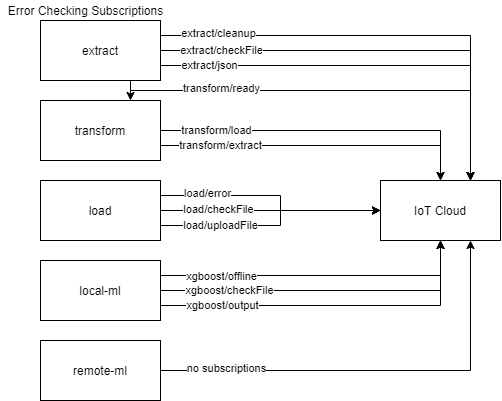
\includegraphics[width=0.75\linewidth]{pages/Chapter4/Chapter 4 Images/LambdaFns/iot_cloud_mqqt.png}
    \caption{Subscriptions from Lambda to IoT Cloud Service for Debugging and Error Checking}
    \label{fig:cloud_mqqt_layer}
\end{figure}

Once the subscriptions have been setup within the Greengrass group as shown in Figure \ref{fig:setup_subs}. It shows the \textit{src} and \textit{dest} addresses for the subscription topic. Any publishes made by the Extract Lambda function will be seen by the IoT Cloud for testing and is discussed further in the testing section.

\begin{figure}[ht]
    \centering
    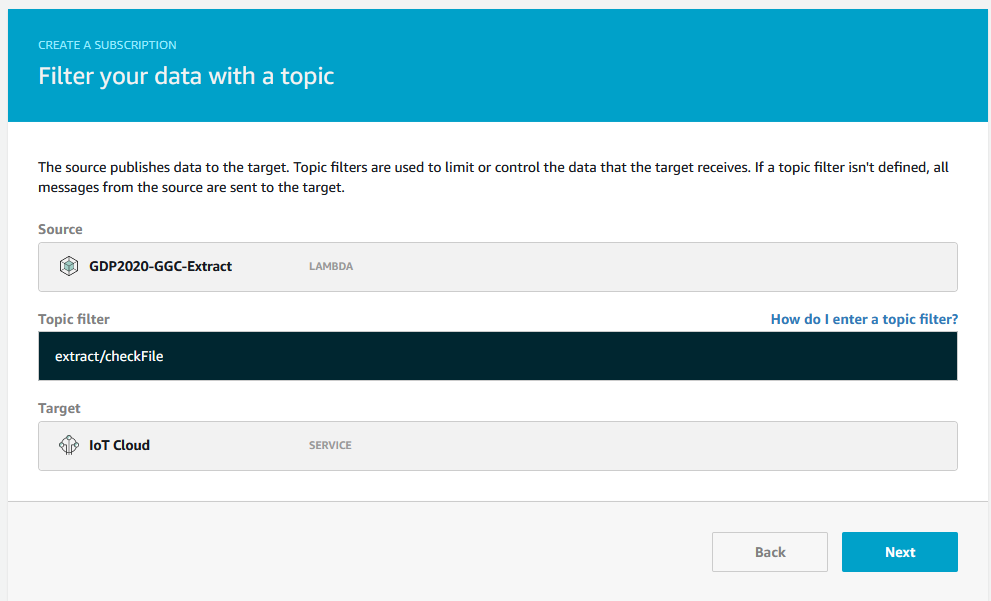
\includegraphics[width=0.75\linewidth]{pages/Chapter4/Chapter 4 Images/setting_up_subscription.png}
    \caption{How the 'extract/checkFile' subscription was setup to send data from the Extract Lambda to IoT Cloud.}
    \label{fig:setup_subs}
\end{figure}

Messages being sent to the IoT Cloud can be seen via the 'Test' tab in the IoT Core dashboard. First the topic to be observed must be entered into the text-box labeled \textit{Subscription Topic}, then the \textit{Display payloads as strings} option should be selected under \textit{MQTT payload display}. Error messages from the Python script can also be captured using \textit{Try} and \textit{Except} blocks to catch and then send any exceptions to the IoT Cloud for easy debugging. This setup is seen in Figure \ref{fig:mqqt_testing_setup}.

\begin{figure}[ht]
    \centering
    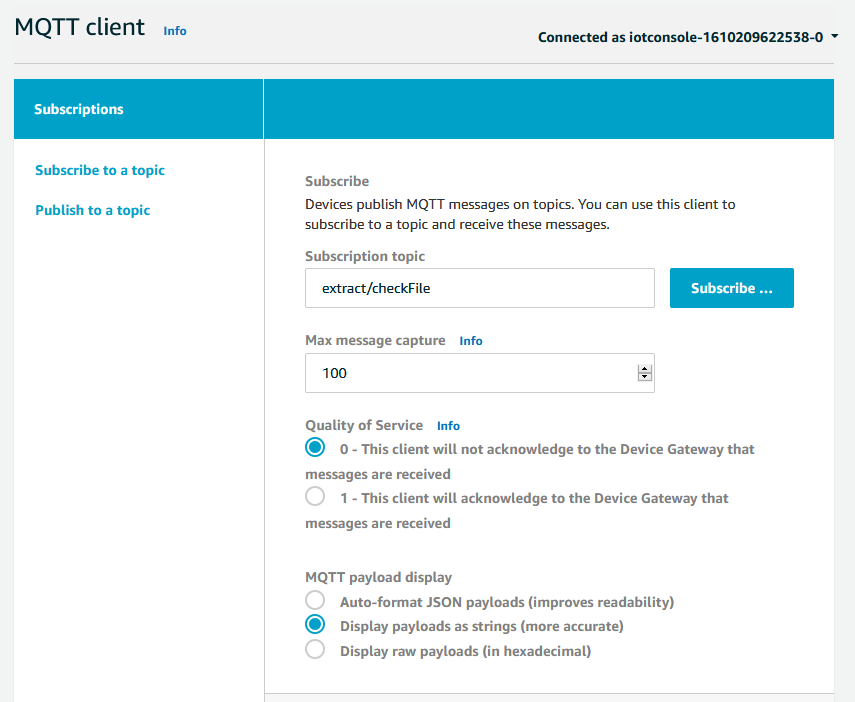
\includegraphics[width=0.75\linewidth]{pages/Chapter4/Chapter 4 Images/setting_up_mqqt_for_test.png}
    \caption{How MQTT Packages can be setup for testing}
    \label{fig:mqqt_testing_setup}
\end{figure}


The above subscriptions were only used for debugging. To send real-time data to the Web-Server application, the subscriptions and topics seen in Figure \ref{fig:mqqt_to_web_app} were setup.

\begin{figure}[ht]
    \centering
    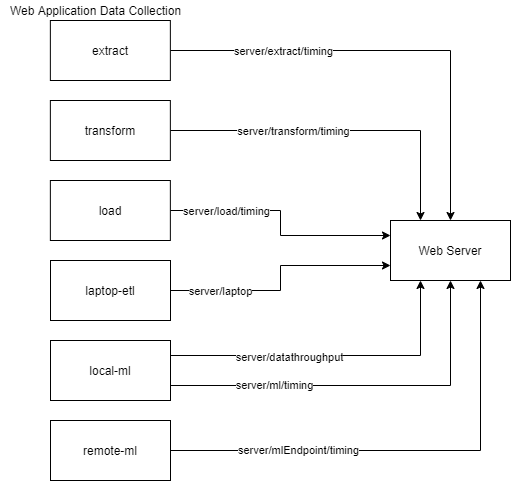
\includegraphics[width=0.7\linewidth]{pages/Chapter4/Chapter 4 Images/nodejs_mqqt.png}
    \caption{Subscriptions and Topics to send data to the Web Application}
    \label{fig:mqqt_to_web_app}
\end{figure}

\subsection{Web Server Application for Live Data Viewing}
\label{nodejs-server}
For this Lambda function, Nodejs is used. Specifically Nodejs 12.x must be used as required by the current version of Greengrass used at the time of this project therefore the runtime must be installed on the edge-device. This is simply a case of downloading the nodejs12.x runtime and storing it on the Edge Devices' \textit{usr/bin/} directory under \textit{nodejs12.x}. This procedure is part of the official documentation regarding Node JS Lambda functions and can be found in more detail on the GitHub page \cite{aws_greengrass_nodejs12_ghub}.

Once this is setup, it is possible to use NodeJS Lambda functions in the Greengrass Group. For the web application, the design choices which needed to be implemented are shown in Figure \ref{fig:web_app_design}. From this, it is understood how each section must be laid out on the Web Server. The central piece will contain a graph to show the data throughput values. Timing of each Lambda function and functions within them will also be shown on the right hand-side of the graph. Then a table with data parameters and classification of the data using the ML model will be shown at the bottom. New data will always be pushed to the top of the table with a maximum of 10 items, so the last table item must be removed.

\begin{figure}[ht]
    \centering
    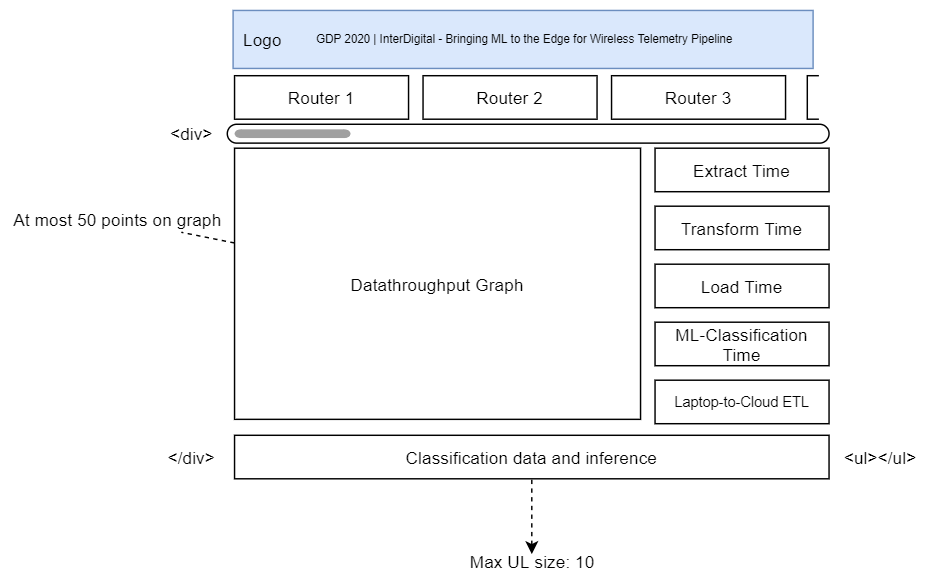
\includegraphics[width=1\linewidth]{pages/Chapter4/Chapter 4 Images/web_app_design.png}
    \caption{Design to be Implemented For Web Application}
    \label{fig:web_app_design}
\end{figure}

In order to set this up, first the back-end of the server must be developed. Using NodeJS for the back-end and Bootstrap \cite{mark_otto_2021}, a HTML/CSS/Javascript package that allows easy website UI/UX elements to be generated can be used to develop the front-end. 

As per all the Lambda functions, anytime a message via a subscription to a topic is received by a Lambda function, a function handler is executed. Most of the time this function handler simply returns without doing anything. In order to process the messages received with the timing and classification data as it is sent in real time, the function handler here is used to process new incoming data. A basic block-level diagram that explains the back-end very simply can be seen in \ref{fig:web_app_block_diagram.} 
The first row of blocks, shows how the function\_handler() operates. When the MQTT package arrives, all the data is stored in the event object, which is passed into the function as a parameter. The event object can then be checked for a \textit{Key} value. The key value indicates what data is contained within the object, and hence letting the program know from which other Lambda function it arrived from. From this, data is extracted and pushed onto the appropriate buffer. This way if a large batch of data is suddenly received from another Lambda, all of it will be shown and processed.

Upon the initialisation of the Lambda function, which would be at the start of the Greengrass Core, the web-server starts, the function handler for every new socket connection is also attached. A loop would also be triggered every \textit{n} seconds, set to five for most purposes as the router data can only be collected every five seconds. In this loop, every data buffer is checked and if any data is present, it is popped off of the buffer and sent to the front-end. To send data in real-time to the front-end from the server back-end, the package socket.io allows seamless integration between the two stack layers. In this case, a simple \textit{sockets.emit} is used to broadcast data to all open connected clients to the server. There are approximately 8  data buffers to handle all data from the various edge-node based Lambda functions.

\begin{figure}[ht]
    \centering
    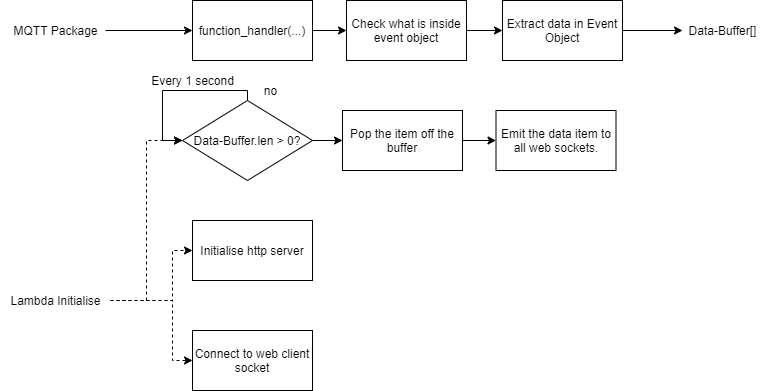
\includegraphics[width=1\linewidth]{pages/Chapter4/Chapter 4 Images/node_web_app.png}
    \caption{Block level diagram explaining systems on the back-end of the Web Server}
    \label{fig:web_app_block_diagram.}
\end{figure}

When the data arrives at the front-end, with the usage of IDs in different HTML tags, it is possible to edit the data within the HTML tag. Since the socket.io emits on a certain keyword. A function is attached to run upon reception of the message with the data from the back-end. The function uses the \textit{document.getElementByID(...)} to edit the text values within the data to the timing values sent by the Lambda functions. The excerpt in Listing \ref{lst:read_socket_data} shows this off.

\begin{lstlisting}[language=HTML, label={lst:read_socket_data}, caption={Reading data sent from the sockets.io connection from the server back-end and editing the front-end HTML page.}]
socket.on('extractTiming', function(extractTiming) {
   let sum = extractTiming.data.DataThroughput + 
        extractTiming.data.PSRetry + extractTiming.data.ChannelStats 
        + extractTiming.data.Assocsta
        + extractTiming.data.PacketetRequested;
        
    document.getElementById('dataTPTime').innerHTML = "DataThroughput.json: <b>" +
        extractTiming.data.DataThroughput.toPrecision(4)+ "s</b>.";
        
    document.getElementById('psRetryTime').innerHTML = "PSRetry.json: <b>" +
        extractTiming.data.PSRetry.toPrecision(4)+ "s</b>.";
        
    document.getElementById('channelStatsTime').innerHTML = "ChannelStats.json: <b>" +
        extractTiming.data.ChannelStats.toPrecision(4)+ "s</b>.";
        
    document.getElementById('assocstaTime').innerHTML = "assocsta.json: <b>" +
        extractTiming.data.Assocsta.toPrecision(4)+ "s</b>.";
        
    document.getElementById('packetReqTime').innerHTML = "PacketRequested.json: <b>" +
        extractTiming.data.PacketetRequested.toPrecision(4)+ "s</b>.";
        
    document.getElementById('extract-time').innerHTML = "Total Extract-Fn Time: <b>"
        + sum.toPrecision(4)+"s</b>";
});
\end{lstlisting}

The code in Listing \ref{lst:read_socket_data} allows for the data shown in Figure \ref{fig:real_time_data_front_end} in bold to be edited in real-time to show the data. First the ID is selected and then the \textit{innerHTML} value is changed to include the type of data and then the timing data is passed via the sockets connection. This listing shows how displayed HTML values can be changed for the Extract Lambda function. The total extract function time, and each data table extraction timing is displayed.

\begin{figure}[ht]
    \centering
    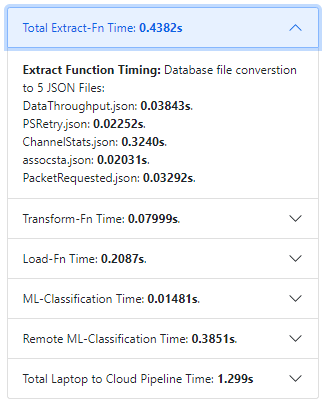
\includegraphics[width=0.5\linewidth]{pages/Chapter4/Chapter 4 Images/newTiming.PNG}
    \caption{Real-time data from Lambda functions to front-end of the Web Application}
    \label{fig:real_time_data_front_end}
\end{figure}

The real-time graph operates in a similar way, where a function is attached to react to messages along a socket.io receive connection. However, rather than editing any given HTML event, the ChartJS \cite{chart_js} package allows a managed real-time graphing application to be embedded onto the website. It also includes appending and removing of data points on the graph in real-time. By using the provided functions this can be done as shown in Listing \ref{lst:append_graph_data_web_app}.

\begin{lstlisting}[language=HTML, caption={How data is updated and removed from the data throughput graph placed centrally in the Web App.}, label={lst:append_graph_data_web_app}]
socket.on('dataTP', function(dataTP) {
    // console.log(dataTP);
    document.getElementById("datatp").innerHTML = dataTP.data;
    time += 0.2;
    addData(myChart,''+time.toPrecision(4)+'s', dataTP.data, 0)
    // console.log("Data queue length is: " + myChart.data.datasets[0].data.length)
    if (myChart.data.datasets[0].data.length > 50) {
        removeData(myChart);
    }
    // $("#datatp").html("currentTP: " + dataTP);
});

\end{lstlisting}

The final implementation of the web application is shown in Figure \ref{fig:impl_web_app}. It follows very closely the design shown in Figure \ref{fig:web_app_design}.

\begin{figure}[ht]
    \centering
    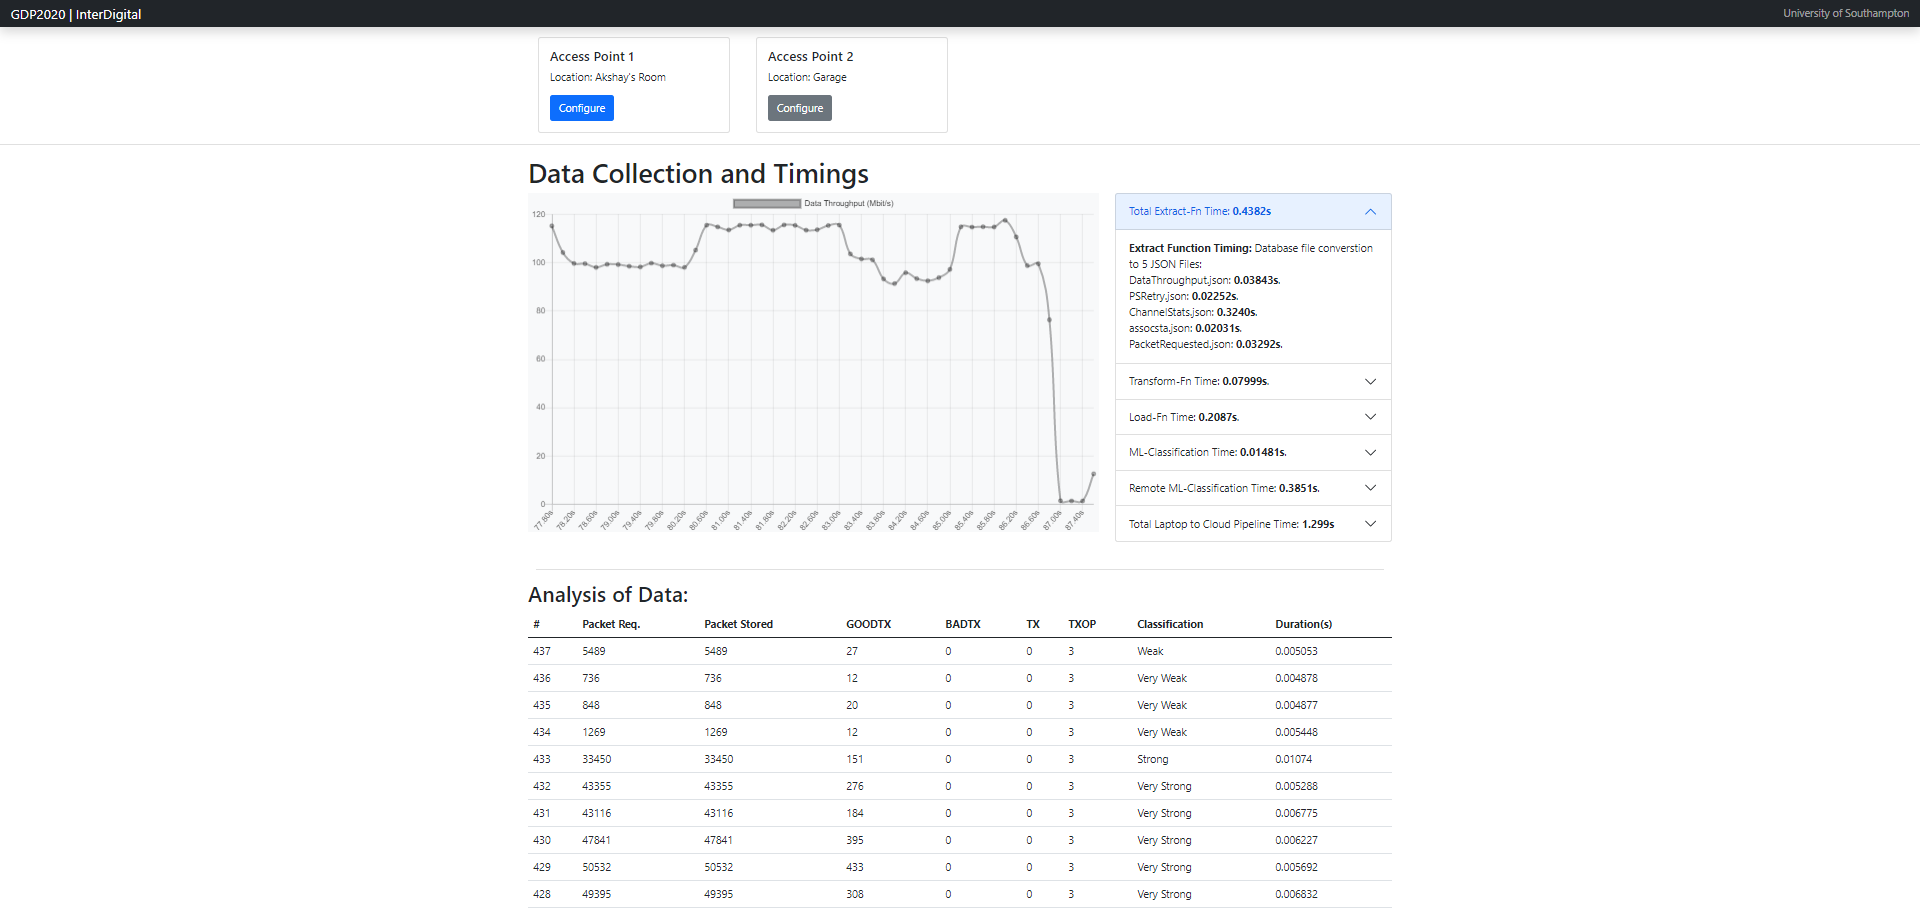
\includegraphics[width=1\linewidth]{pages/Chapter4/Chapter 4 Images/newWebApp.PNG}
    \caption{Fully implemented web application design - The full scale figure can be found in Appendix Section \ref{appendix:full_web_app}}
    \label{fig:impl_web_app}
\end{figure}


\section{Edge Node Technology Exploration - AdvantEDGE} %Syuhada's Section
\subsection{AdvantEDGE Implementation}
The mobile edge emulation platform requires a system that runs on bare Linux operating system (OS) or within virtual machines, and may be installed on a single Kubernetes (K8s) node or a cluster of K8s nodes. The system requirements to install AdvantEDGE include building the runtime environments – Ubuntu, Dockers, Kubernetes, Helm and NVIDIA GPU support. With the system setup, one can clone AdvantEDGE repositories into local host before installing and configure the meepctl tool, a command-line interface (CLI) applications to control the platform. 
Configuring meepctl to the node’s IP address and the directory on the local host, AdvantEDGE binaries can be built to generate the micro-services, as well as the front-end web application. AdvantEDGE micro-services fall into two categories: core and dependencies. Prior to deploying AdvantEDGE core components, dependencies to create micro-services required to run AdvantEDGE can be deployed onto K8s cluster with the meepctl tool and then dockerize these micro-services into container images to be stored into a configured Docker registry. The platform GUI then can be accessed through the standard browser.

To emulate the physical system model, a scenario of the network model can be built by configuring each of the elements needed such as the Internet Cloud, operator, zones, PoA and the edge nodes,  connecting the simulation platform to the physical running native edge application on the server. 

This edge native application is the same Python script used in the AWS IoT Greengrass edge node that is able to extract, transform and load the data before sending them off to the distant cloud. However, prior to connecting the edge application to the AdvantEDGE, the Python application is required to be containerized into Docker image and stored in the Docker registry. Dockerfile, a text document without the extension that contains all the commands a user could call on the command line to assemble an image, has to be created, placed together in the same directory as the Python script and requirement.txt. Requirement.txt is a file that contains the dependencies that the Python script needs to run successfully. This file can be first generated on the command line using \textit{“pip freeze \textgreater\textgreater requirement.txt”}. 

\begin{figure}[ht]
    \centering
    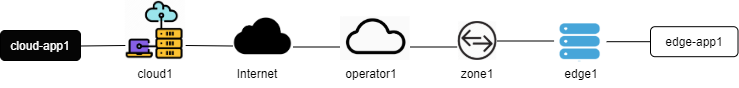
\includegraphics[width=1\linewidth]{pages/Chapter4/Chapter 4 Images/Scenario.png}
    \caption{Scenario created in AdvantEDGE to emulate the physical network topology}
    \label{fig:AdvantEDGE_scenario}
\end{figure}

On AdvantEDGE web GUI, a scenario is created as shown in Figure \ref{fig:AdvantEDGE_scenario}.
The cloud and edge application are connected to the real applications through the configuration where detailed specifications such as group container name, port, protocol, command and arguments need to be provided before deploying the scenario into the sandbox. The scenario then can be deployed once the button on the top right turns green, indicating the server is all good. When executed, one can set the source node and the destination node, to measure the latency, data throughput and traffic metrics in between the nodes after configuring the elements’ network characteristics which can indirectly configure the router. It displays instantaneous measurements for round-trip ping time on the graph if we select to display it on the Network Metrics Point-to-Point.

\begin{lstlisting}[language=Python, caption={Example of Dockerfile}, label={lst:dockerfile}]
# Select the base image to build the new image on top
FROM python:3

# Define the default working directory for any RUN, CMD, ENTRYPOINT, COPY and ADD command
WORKDIR /usr/src/app

# Copy files from Docker host to your Docker image
COPY requirements.txt ./

# Install Python modules required in the requirement.txt
RUN pip install --no-cache-dir -r requirements.txt

# Copy the entire project, recursively into the container for the build
COPY . .

# Execute when the container starts
CMD [ "python", "./python_application.py" ]


# In command line shell to build the image from Dockerfile.
# my-python-app is the name of Docker image that one wants to assign 
$ docker build -t my-python-app .
$ docker run -it --rm --name my-running-app my-python-app

\end{lstlisting}


